\documentclass[11pt,a4paper]{article}
\usepackage{enumitem}
\usepackage{graphicx}           % Extended \includegraphics         
\usepackage[reqno]{amsmath}            % Higher mathematics
\usepackage{hyperref}           
\usepackage[margin = 0.5in]{geometry}
\usepackage{float}
\usepackage{amssymb}            % special math fonts
\usepackage{amsmath}
\usepackage{siunitx}
\usepackage{enumitem}
\usepackage{cancel}
\usepackage{braket}
\usepackage{tikz}
\usepackage{pgfplots}
\usepackage[final]{pdfpages}
\usepackage{physics}
\usepackage{subcaption}
\usepackage{bbm}
\usepackage{rotating}
\usepackage{listings}
\usepackage{color}

\makeatletter
\renewcommand*\env@matrix[1][*\c@MaxMatrixCols c]{%
  \hskip -\arraycolsep
  \let\@ifnextchar\new@ifnextchar
  \array{#1}}
\makeatother

\definecolor{codegreen}{rgb}{0,0.6,0}
\definecolor{codered}{rgb}{0.6,0,0}
\definecolor{codeblue}{rgb}{0,0,0.6}
\definecolor{codegray}{rgb}{0.5,0.5,0.5}
\definecolor{codepurple}{rgb}{0.58,0,0.82}
\definecolor{backcolour}{rgb}{0.95,0.95,0.92}
 
\lstdefinestyle{mystyle}{
    backgroundcolor=\color{backcolour},   
    commentstyle=\color{codered},
    keywordstyle=\color{codeblue},
    numberstyle=\tiny\color{codegray},
    stringstyle=\color{codegreen},
    basicstyle=\footnotesize,
    breakatwhitespace=false,         
    breaklines=true,                 
    captionpos=b,                    
    keepspaces=true,                 
    numbers=left,                    
    numbersep=5pt,                  
    showspaces=false,                
    showstringspaces=false,
    showtabs=false,                  
    tabsize=2
}
 
\lstset{style=mystyle}

%\tikzexternalize[optimize=false,prefix=PREFIX]

\pgfplotsset{compat = 1.13}

\newcommand{\h}{\hat}
\newcommand{\hham}{\hat{\mathcal{H}}}

\begin{document}


\title{\bf PHYC90010 - Statistical Mechanics Assignment 3}
\author{Mitchell de Zylva - 756539}
\maketitle



\begin{center}
\vspace{1cm}
\rule{145mm}{0.5mm}
\vspace{1cm}
\end{center}
\tableofcontents
\newpage
%\input{/home/part3/mylatex/preamble}
\newpage

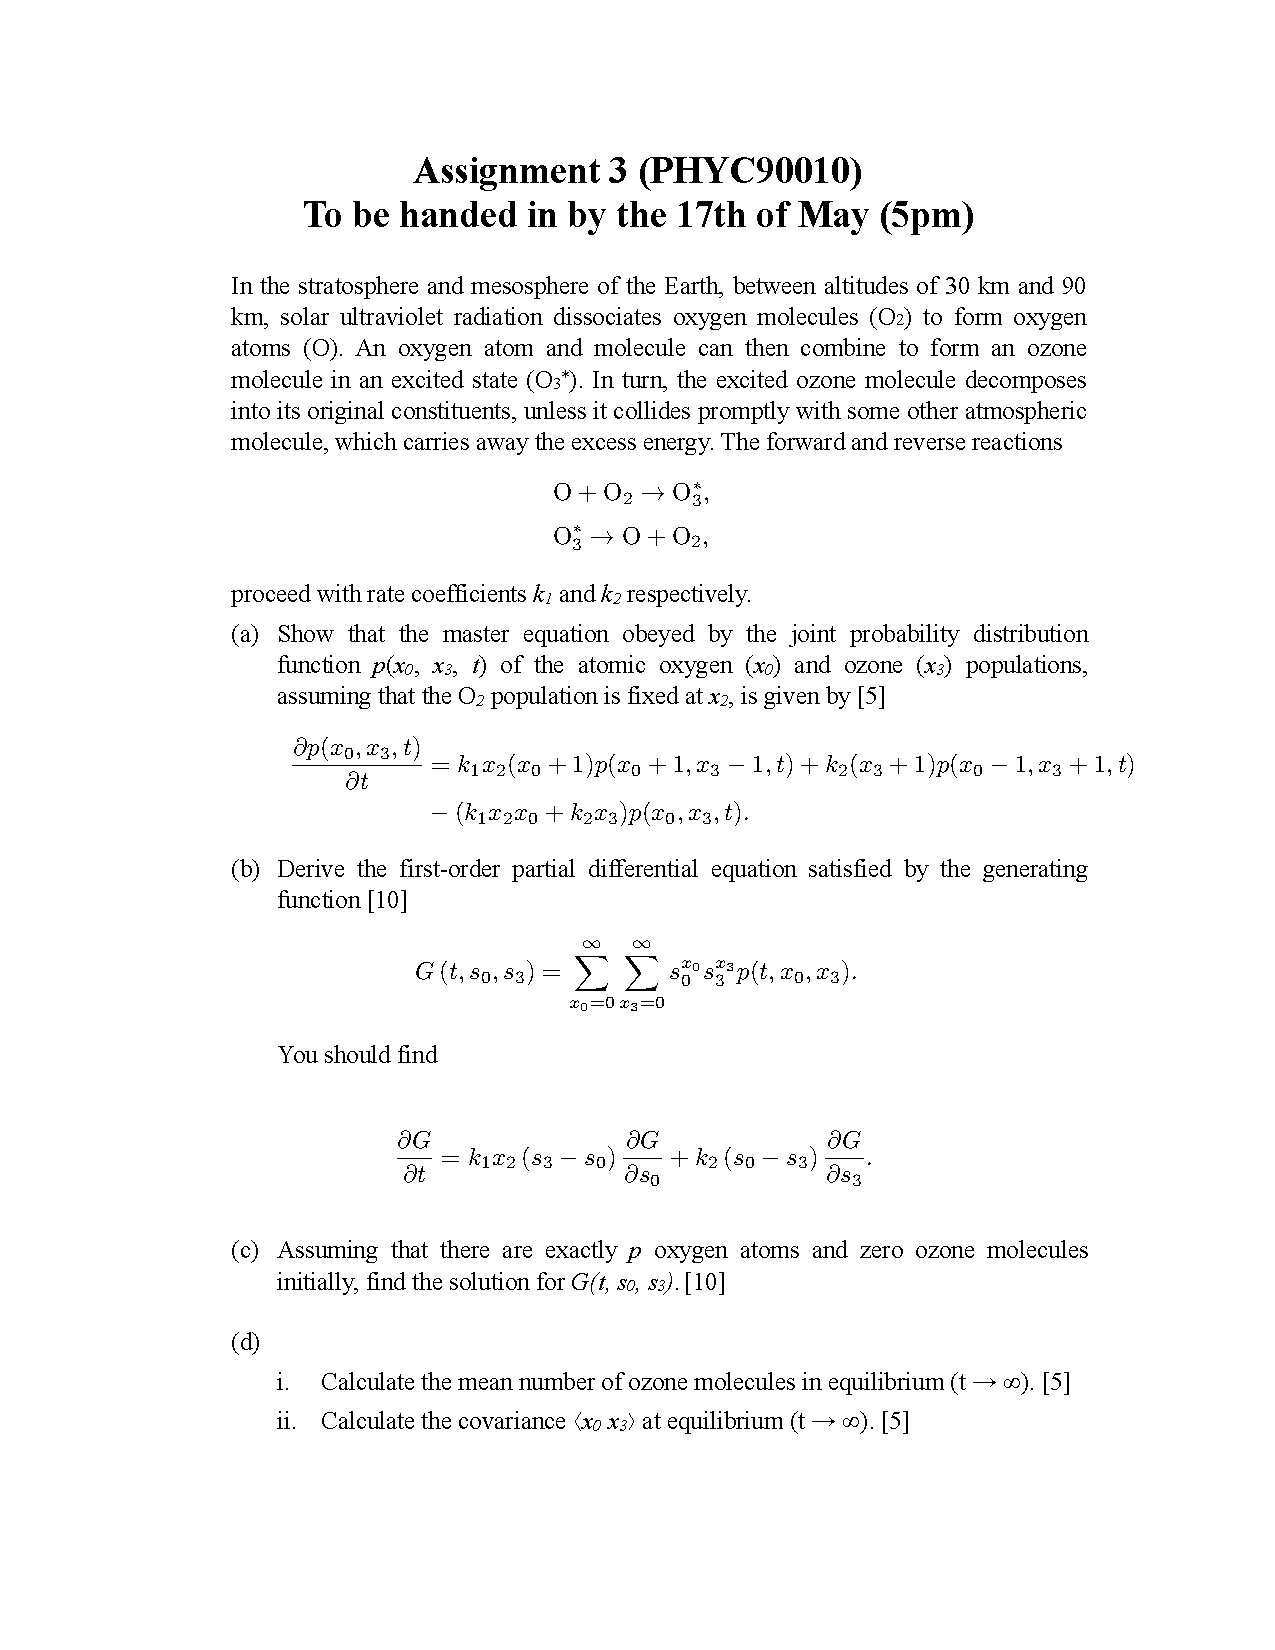
\includepdf[pages=-]{/home/mitchell/Documents/masters/statmech/third/Assign3_2019.pdf}


%%%%%%%%%%%%%%%%%%%%%%%%%%%%%%%%%%%%%%%%%%%%%%%%%%%%%%%%%%%%%%%%%%%%%%
\section{Question 1}
\label{sec:question1}
%%%%%%%%%%%%%%%%%%%%%%%%%%%%%%%%%%%%%%%%%%%%%%%%%%%%%%%%%%%%%%%%%%%%%%
%%%%%%%%%%%%%%%%%%%%%%%%%%%
\subsection{Question 1 - (a)}
\label{sec:question1:subsec:parta}
%%%%%%%%%%%%%%%%%%%%%%%%%%%
We know that by definition, $\pdv{p(x_0,x_3,t)}{t}$ is given by subtracting the Rate leaving $x_0$ and $x_3$ from the Rate entering $x_0$ and $x_3$. We know that the rate entering $x_0$ is given by 
$$ k_2 (x_3 + 1) p(x_0-1,x_3+1,t),  $$
and the rate leaving $x_0$ is given by 
$$ k_1 x_0 x_2 p(x_0,x_3,t).  $$
Similarly, the rate entering $x_3$ is given by 
$$ k_1 x_2 (x_0+1) p(x_0+1,x_3-1,t), $$
and the rate leaving $x_3$ is given by 
$$ k_2 x_3 p(x_0,x_3,t) .$$
By combinging these, we see that this makes the rate of change of the probability function 
\begin{equation}\label{eq:master_eq}
\pdv{p(x_0,x_3,t)}{t} = k_1 x_2 (x_0+1) p(x_0+1,x_3-1,t) + k_2 (x_3+1) p(x_0-1,x_3+1,t) - (k_1 x_0 x_2 + k_2 x_3) p(x_0,x_3,t)
\end{equation}
as required.
%%%%%%%%%%%%%%%%%%%%%%%%%%%
\subsection{Question 1 - (b)}
\label{sec:question1:subsec:partb}
%%%%%%%%%%%%%%%%%%%%%%%%%%%
By using a generating function of the form 
\begin{equation}
G(t,s_0,s_3) = \sum_{x_{0}=0}^{\infty} \sum_{x_{3}=0}^{\infty} s_0^{x_0} s_3^{x_3} p(t,x_0,x_3)
\end{equation}
and substituing it into \eqref{eq:master_eq}, we can pass the partial differential through the sums, and assuming that the $s_0$ and $s_3$ terms are constants in time, we see that
\begin{align*}
\pdv{G}{t} = & \sum_{x_0=0}^{\infty} \sum_{x_3=0}^{\infty} s_0^{x_0} s_3^{x_3} \pdv{p}{t} \\
= & k_1 x_2 \sum_{x_0=0}^{\infty} \sum_{x_3=0}^{\infty} (x_0 + 1) s_0^{x_0} s_3^{x_3} p(x_0+1,x_3-1,t) + k_2 \sum_{x_0=0}^{\infty} \sum_{x_3=0}^{\infty} (x_3+1) s_0^{x_0} s_3^{x_3} p(x_0-1,x_3+1,t) \\ 
& - k_1 x_2 \sum_{x_0=0}^{\infty} \sum_{x_3=0}^{\infty} x_0 s_0^{x_0} s_3^{x_3} p(x_0,x_3,t) + k_2 \sum_{x_0=0}^{\infty} \sum_{x_3=0}^{\infty} x_3 s_0^{x_0} s_3^{x_3} p(x_0,x_3,t). 
\end{align*}
We can now change the terminals on the summation by making the substitutions, $x_0 \rightarrow x_0 -1 $ in the first term, and $x_3 \rightarrow x_3 - 1$ in the second term, the above becomes
\begin{align*}
= & k_1 x_2 \sum_{x_0=-1}^{\infty} \sum_{x_3=0}^{\infty} x_0  s_0^{x_0-1} s_3^{x_3} p(x_0,x_3-1,t) + k_2 \sum_{x_0=0}^{\infty} \sum_{x_3=-1}^{\infty} x_3 s_0^{x_0} s_3^{x_3-1} p(x_0-1,x_3,t) \\ 
& - k_1 x_2 \sum_{x_0=0}^{\infty} \sum_{x_3=0}^{\infty} x_0 s_0^{x_0} s_3^{x_3} p(x_0,x_3,t) + k_2 \sum_{x_0=0}^{\infty} \sum_{x_3=0}^{\infty} x_3 s_0^{x_0} s_3^{x_3} p(x_0,x_3,t) .
\end{align*}
Now, if we make similar substitutions, where $x_3 \rightarrow x_3 + 1$ for the first term, and $x_0 \rightarrow x_0 +1 $ for the second term, this becomes 
\begin{align*}
= & k_1 x_2 \sum_{x_0=-1}^{\infty} \sum_{x_3=1}^{\infty} x_0 s_0^{x_0-1} s_3^{x_3+1} p(x_0,x_3,t) + k_2 \sum_{x_0=1}^{\infty} \sum_{x_3=-1}^{\infty} x_3 s_0^{x_0+1} s_3^{x_3-1} p(x_0,x_3,t) \\ 
& - k_1 x_2 \sum_{x_0=0}^{\infty} \sum_{x_3=0}^{\infty} x_0 s_0^{x_0} s_3^{x_3} p(x_0,x_3,t) + k_2 \sum_{x_0=0}^{\infty} \sum_{x_3=0}^{\infty} x_3 s_0^{x_0} s_3^{x_3} p(x_0,x_3,t) .
\end{align*}
Now, we note that the probability distribution function cannot have any non-zero value for any $x$ value less than zero. Practically, this means 
\begin{align*}
p(x_0,-1,t) &= 0 \text{ and }\\
p(-1,x_3,t) &= 0.
\end{align*}
Taking this now term by term, we can shift the terminals on the sum back, so that we can collect terms inside one set of sums. 
\paragraph{First Term}
We can shift the $x_0$ sum in the first term by appealing to the nature of the probability distribution, and we can shift the $x_3$ sum by separating out the 
\begin{align*}
k_1 x_2 \sum_{x_0=-1}^{\infty} \sum_{x_3=1}^{\infty} x_0 s_0^{x_0-1} s_3^{x_3+1} p(x_0,x_3,t) &= k_1 x_2 \sum_{x_0=0}^{\infty} \sum_{x_3=1}^{\infty} x_0 s_0^{x_0-1} s_3^{x_3+1} p(x_0,x_3,t) \\ 
&= k_1 x_2 s_3 \sum_{x_0=0}^{\infty} \sum_{x_3=0}^{\infty} x_0 s_0^{x_0-1} s_3^{x_3}  p(x_0,x_3,t).
\end{align*}
\paragraph{Second Term}
For the second term, we can perform the same operations on the other variable, giving
\begin{align*}
k_2 \sum_{x_0 = 1}^\infty \sum_{x_3=-1}^\infty x_3 s_0^{x_0+1} s_3^{x_3-1} p(x_0,x_3,t) &= 
k_2 \sum_{x_0 = 1}^\infty \sum_{x_3=0}^\infty x_3 s_0^{x_0+1} s_3^{x_3-1} p(x_0,x_3,t) \\
&= k_2 s_0 \sum_{x_0 = 0}^\infty \sum_{x_3=0}^\infty x_3 s_0^{x_0} s_3^{x_3-1} p(x_0,x_3,t).
\end{align*}
\paragraph{Third Term}
For the third term, we can simply reshuffle the powers of $s_0$ to show 
\begin{align*}
- k_1 x_2 \sum_{x_0 = 0}^\infty \sum_{x_3 = 0}^\infty x_0 s_0^{x_0} s_3^{x_3} p(x_0,x_3,t) = 
-k_1 x_2 s_0 \sum_{x_0 = 0}^\infty \sum_{x_3 = 0}^\infty x_0 s_0^{x_0-1} s_3^{x_3}.  p(x_0,x_3,t)
\end{align*}
\\
\paragraph{Fourth Term}
Simillarly, for the fourth term, we can simply reshuffle the powers of $s_3$ to show 
\begin{align*}
- k_2 \sum_{x_0 = 0}^\infty \sum_{x_3 = 0}^\infty x_3 s_0^{x_0} s_3^{x_3} p(x_0,x_3,t) = 
-k_2 s_3 \sum_{x_0 = 0}^\infty \sum_{x_3 = 0}^\infty x_3 s_0^{x_0} s_3^{x_3-1}  p(x_0,x_3,t).
\end{align*}
Combining all four terms, this becomes 
\begin{align*}
=& k_1 x_2 s_3 \sum_{x_0=0}^{\infty} \sum_{x_3=0}^{\infty} x_0 s_0^{x_0-1} s_3^{x_3}  p(x_0,x_3,t) -k_1 x_2 s_0 \sum_{x_0 = 0}^\infty \sum_{x_3 = 0}^\infty x_0 s_0^{x_0-1} s_3^{x_3}  p(x_0,x_3,t)  \\
& + k_2 s_0 \sum_{x_0 = 0}^\infty \sum_{x_3=0}^\infty x_3 s_0^{x_0} s_3^{x_3-1} p(x_0,x_3,t)
-k_2 s_3 \sum_{x_0 = 0}^\infty \sum_{x_3 = 0}^\infty x_3 s_0^{x_0} s_3^{x_3-1}  p(x_0,x_3,t)
\\
=& k_1 x_2 (s_3 -s_0) \sum_{x_0 = 0}^\infty \sum_{x_3 = 0}^\infty x_0 s_0^{x_0-1} s_3^{x_3} p(x_0,x_3,t) + k_2 (s_0 -s_3) \sum_{x_0 = 0}^\infty \sum_{x_3 = 0}^\infty x_3 s_0^{x_0} s_3^{x_3-1}  p(x_0,x_3,t) \\
=& k_1 x_2 (s_3 - s_0) \pdv{G}{s_0} + k_2 (s_0 - s_3) \pdv{G}{s_3}, 
\end{align*}
as required.
%%%%%%%%%%%%%%%%%%%%%%%%%%%
\subsection{Question 1 - (c)}
\label{sec:question1:subsec:partc}
%%%%%%%%%%%%%%%%%%%%%%%%%%%
Now, this yields a partial differential equation, which can be solved by the method of characteristics. This is apparently the purview of Applied Mathematical Modelling, which I have not done, so I am attempting this for the first time. 
\par We consider a curve in $r-t$ space which is constant, and therefore make a change of variables from $t$ to $r$, which gives us a differential equation where
$$ \dv{G}{r} = \pdv{G}{t} \dv{t}{r} + \pdv{G}{s_0} \dv{s_0}{r} + \pdv{G}{s_3} \dv{s_3}{r} $$
Since the curve we are considering is constant, the solution will have the form
$$ G(t,s_0,s_3) = [s_0(t=0)]^p $$
This gives three characteristic equations 
\begin{align}
\dv{t}{r} &= 1 \ \Rightarrow t(r) = r \label{eq:char:t} \\ 
\dv{s_0}{r} &= - k_1 x_2 (s_3 - s_0) \label{eq:char:s_0} \\
\dv{s_3}{r} &= - k_2 (s_0 - s_3)  \label{eq:char:s_3}
\end{align}
The \eqref{eq:char:s_0} and \eqref{eq:char:s_3} are coupled ODE's, which we can solve by treating them as a system of equations. Reexpressing them in terms of $a = - k_1 x_2 $ and $b= -k_2$ for convenience they become
\begin{align}
\dv{s_0}{r} &= a (s_3 - s_0) \label{eq:sys:one} \\
\dv{s_3}{r} &= b (s_0 - s_3) \label{eq:sys:two}
\end{align} 
Now, rearranging \eqref{eq:sys:one}, we see
\begin{equation}\label{eq:s_0}
s_0 = s_3 - \frac{1}{a} \dv{s_0}{r} .
\end{equation}
Now, if we substitute this into \eqref{eq:sys:two}, it becomes 
\begin{align*}
\dv{s_3}{r} &= b( \cancel{s_3} - \frac{1}{a} \dv{s_0}{r} - \cancel{s_3} ) \\
\dv{s_3}{r} &= - \frac{b}{a} \dv{s_0}{r} \\
\end{align*}
\begin{equation}\label{eq:s_3}
\Rightarrow s_3 = -\frac{b}{a} s_0 + C_1 
\end{equation}
Substituting \eqref{eq:s_3} into \eqref{eq:sys:one} gives
\begin{align*}
\dv{s_0}{r} &= a (- \frac{b}{a} s_0 + C_1 - s_0) \\
&= - b s_0 + a C_1 - a s_0 \\
\dv{s_0}{r} &= - (a+b) s_0 + a C_1 \\
\frac{\dv{s_0}{r}}{a C_1 - (a+b) s_0} = 1 \\
\Rightarrow - \frac{\log(a C_1 - (a+b) s_0(r)) }{a+b} &= r + C_2 \\ 
\end{align*}
Note that above, we obtain $s_3(r)$ from \eqref{eq:s_3} for free.
\begin{align}
\Rightarrow s_0(r) &= \frac{a}{a+b} C_1 +  C_2 e^{- (a+b) t} \label{eq:s_0:r}\\
\Rightarrow s_3(r) &= \frac{a}{a+b} C_1 -\frac{b}{a} C_2 e^{- (a+b) t} \label{eq:s_3:r}
\end{align}
Now, rearranging \eqref{eq:s_0:r} and \eqref{eq:s_3:r}, and setting $a+b=\beta$ for convenience, we can obtain a value for $C_2$, and we get the expression for $C_1$ from \eqref{eq:s_3}
\begin{align*}
s_3 - s_0 &= \frac{b}{a} C_2 e^{-\beta t} + C_2 e^{-\beta t} \\
&= \frac{a + b}{a} C_2 e^{-\beta t} \\
\Rightarrow C_2 &= - \frac{a}{\beta} (s_3 - s_0) e^{-\beta t} \\
\Rightarrow C_1 &= s_3 + \frac{b}{a} s_0
\end{align*} 
Now, since we want to find the solution on the constant curve, and we know that the initial number of oxygen atoms is $p$, then the solution will be some constant value, defined by the value of the generating function for that condition. Therefore
\begin{align*}
G(t,s_0,s_3) &= \left[ s_0(t=0) \right]^p \\
&= \left[ \frac{a}{\beta} C_1 - C_2 \right]^p \\
&= \left[ \frac{a}{\beta} (s_3 + \frac{b}{a} s_0) - \frac{a}{\beta} (s_3 - s_0) e^{-\beta t}\right]^p \\
&= \left[ \frac{(-b s_0 - a s_3) (1 - e^{-\beta t})}{\beta} + s_0 e^{-\beta t} \right]^p \\
&= \left[ \frac{(k_2 s_0 + k_1 x_2 s_3) (1 - e^{-\beta t})}{\beta} + s_0 e^{-\beta t} \right]^p 
\end{align*}
%%%%%%%%%%%%%%%%%%%%%%%%%%%
\subsection{Question 1 - (d)}
\label{sec:question1:subsec:partd}
%%%%%%%%%%%%%%%%%%%%%%%%%%%

%%%%%%%%%%%%%%%%%%%%%%%%%%%
\subsubsection{Question 1 - (d) - i}
\label{sec:question1:subsec:partd:subsub:i}
%%%%%%%%%%%%%%%%%%%%%%%%%%%
We can compute the mean number of ozone molecules by using the generating function 
\begin{align*}
\left\langle x_3 \right\rangle &=  \pdv{G}{s_3}\bigg\rvert_{s_0=s_3=1} \\
&= \pdv{s_3} \left[ \left( \frac{(k_2 s_0 + k_1 x_2 s_3) (1- e^{-\beta t} )}{\beta} + s_0 e^{-\beta t} \right)^p \right] \\
&= p \left( \frac{(k_2 s_0 + k_1 x_2 s_3) (1- e^{-\beta t} )}{\beta} + s_0 e^{-\beta t} \right)^{p-1} \left(\frac{k_1 x_2 (1 - e^{-\beta t} ) }{\beta}\right) \\
&= p \left( \frac{\cancel{\beta} (1- e^{-\beta t} )}{\cancel{\beta}} + s_0 e^{-\beta t} \right)^{p-1} \left(\frac{k_1 x_2 (1 - e^{-\beta t} ) }{\beta}\right) 
\end{align*} 
Now taking the mean in equilibrium, we take the limit where $t \rightarrow \infty$, which becomes
\begin{align*}
\left\langle x_3 \right\rangle \bigg\rvert_{t\rightarrow \infty} &= \lim_{t\rightarrow \infty} \left[ p \left( (1- e^{-\beta t} ) + s_0 e^{-\beta t} \right)^{p-1} \left(\frac{k_1 x_2 (1 - e^{-\beta t} ) }{\beta}\right) \right] \\
&= \left[ p \left( (1 \cancel{-e^{-\beta t}} ) \cancel{+ s_0 e^{-\beta t}} \right)^{p-1} \left(\frac{k_1 x_2 (1 \cancel{- e^{-\beta t} }) }{\beta}\right) \right] \\
&= p [1]^{p-1} \frac{k_1 x_2}{k_2 + k_1 x_2} \\
&= \frac{p k_1 x_2}{k_2 + k_1 x_2}
\end{align*}
%%%%%%%%%%%%%%%%%%%%%%%%%%%
\subsubsection{Question 1 - (d) - ii}
\label{sec:question1:subsec:partd:subsub:ii}
%%%%%%%%%%%%%%%%%%%%%%%%%%%
Similarly, in order to compute the cross correlation, we use the generating function, in the form 
\begin{align*}
\left\langle x_0 x_3 \right\rangle &= \pdv{G}{s_0}{s_3} \bigg\rvert_{s_0=s_3=1} - \left\langle x_0 \right\rangle \left\langle x_3 \right\rangle
\end{align*}
In order to compute this, we first need to find $\left\langle x_0 \right\rangle$, which we do in the same method as above
\begin{align*}
\left\langle x_0 \right\rangle &= \pdv{G}{s_0}\bigg\rvert_{s_0=s_3=1} \\
&= \pdv{s_0} \left[ \left( \frac{(k_2 s_0 + k_1 x_2 s_3) (1- e^{-\beta t} )}{\beta} + s_0 e^{-\beta t} \right)^p \right] \\
&= p \left( \frac{(k_2 s_0 + k_1 x_2 s_3) (1- e^{-\beta t} )}{\beta} + s_0 e^{-\beta t} \right)^{p-1} \left( k_2 (1-e^{-\beta t}) + e^{-\beta t} \right) \\
&= p \left( \frac{\cancel{\beta} (1- e^{-\beta t} )}{\cancel{\beta}} + s_0 e^{-\beta t} \right)^{p-1} \left( \frac{k_2}{\beta} (1-e^{-\beta t}) + e^{-\beta t} \right) 
\end{align*}
Again, finding the long term behaviour gives us 
\begin{align*}
\left\langle x_0 \right\rangle &= \lim_{t\rightarrow \infty} \left[ p \left((1 \cancel{- e^{-\beta t}} ) + \cancel{s_0 e^{-\beta t}} \right)^{p-1} \left( \frac{k_2}{\beta} (1\cancel{-e^{-\beta t}}) + \cancel{e^{-\beta t}} \right) \right] \\
&= p \left[1\right]^{p-1} \frac{k_2}{\beta} \\
&= \frac{p k_2}{\beta} 
\end{align*}
Now, we have to find $\pdv{G}{s_0}{s_3}$. Taking the solution found in \ref{sec:question1:subsec:partd:subsub:ii}, we can see
\begin{align*}
\pdv{G}{s_0}{s_3} &= \pdv{s_0} \left[p \left( \frac{(k_2 s_0 + k_1 x_2 s_3) (1- e^{-\beta t} )}{\beta} + s_0 e^{-\beta t} \right)^{p-1} \left(\frac{k_1 x_2 (1 - e^{-\beta t} ) }{\beta}\right) \right] \\ 
&= p (p-1) \left( \frac{(k_2 s_0 + k_1 x_2 s_3) (1- e^{-\beta t} )}{\beta} + s_0 e^{-\beta t} \right)^{p-2} \left(\frac{k_1 x_2 (1 - e^{-\beta t} ) }{\beta}\right) \left(\frac{k_2}{\beta} (1 - e^{-\beta t}) + e^{-\beta t} \right) 
\end{align*}
Again, taking the behaviour as $t \rightarrow \infty$, this becomes
\begin{align*}
\pdv{G}{s_0}{s_3} \rightarrow & p ( p-1) [1]^{p-2} \frac{k_1 x_2}{\beta} \frac{k_2}{\beta} \\
= & p (p-1) \frac{k_1 k_2 x_2}{\beta^2}
\end{align*}
Now, substituting into our expression for $\left\langle x_0 x_3 \right \rangle$, we see that it becomes
\begin{align*}
\left\langle x_0 x_3 \right \rangle &= p (p-1) \frac{k_1 k_2 x_2}{\beta^2} - \frac{p (k_1 x_2)}{\beta} p \frac{k_2}{\beta} \\
&= p (p-1) \frac{k_1 k_2 x_2}{\beta^2} - \frac{p^2 (k_1 k_2 x_2) }{\beta^2} \\
&= - p \frac{k_1 k_2 x_2}{\beta^2}
\end{align*}
%%%%%%%%%%%%%%%%%%%%%%%%%%%
\subsubsection{Question 1 - (d) - iii}
\label{sec:question1:subsec:partd:subsub:iii}
%%%%%%%%%%%%%%%%%%%%%%%%%%%
Since the answer for the covariance found in \ref{sec:question1:subsec:partd:subsub:iii} is negative, this suggests that the number of ozone molecules and oxygen molecules are anti-correlated at equilibrium. This makes sense, since physically, provided there are only a fixed number of oxygen atoms in the system, the amount of ozone molecules will go up as the number of oxygen molecules go down, and vice-versa. 
\end{document}
